%%%%%%%%%%%%%%%%%%%%%%%%%%%%%%%%%%%%%%%%%
% Journal Article
% LaTeX Template
% Version 2.0 (February 7, 2023)
%
% This template originates from:
% https://www.LaTeXTemplates.com
%
% Author:
% Vel (vel@latextemplates.com)
%
% License:
% CC BY-NC-SA 4.0 (https://creativecommons.org/licenses/by-nc-sa/4.0/)
%
% NOTE: The bibliography needs to be compiled using the biber engine.
% Minor mod to keep all options in one file jc
%%%%%%%%%%%%%%%%%%%%%%%%%%%%%%%%%%%%%%%%%

%----------------------------------------------------------------------------------------
%	PACKAGES AND OTHER DOCUMENT CONFIGURATIONS
%----------------------------------------------------------------------------------------
%
\documentclass[
	letterpaper, % Paper size, use either a4paper or letterpaper
	10pt, % Default font size, can also use 11pt or 12pt, although this is not recommended
	% unnumberedsections, % Comment to enable section numbering
	% twoside, % Two side traditional mode where headers and footers change between odd and even pages, comment this option to make them fixed
]{article}


%----------------------------------------------------------------------------------------
%	CLASS CONFIGURATION
%----------------------------------------------------------------------------------------

\NeedsTeXFormat{LaTeX2e}
% \ProvidesClass{LTJournalArticle}[2023/02/07 LaTeX Templates Journal Article Class v2.0]

\usepackage{etoolbox} % Required for conditional logic and easily changing commands

\newtoggle{unnumberedsections} % Create toggle for a class option
\settoggle{unnumberedsections}{false} % Default value for the class option
\DeclareOption{unnumberedsections}{\settoggle{unnumberedsections}{true}} % Set the class option toggle if the class option was used in the template

\DeclareOption*{\PassOptionsToClass{\CurrentOption}{article}} % Pass through any extra options specified to the base class
\ProcessOptions\relax % Process class options

% \LoadClass[twocolumn]{article} % Load the base class

%----------------------------------------------------------------------------------------
%	REQUIRED PACKAGES AND MISC CONFIGURATIONS
%----------------------------------------------------------------------------------------

\usepackage{graphicx} % Required for including images
\graphicspath{{media/}{./}} % Specifies where to look for included images (trailing slash required)

\usepackage[bottom, hang]{footmisc} % Force footnotes to the bottom of the page and to the left margin
\setlength{\footnotemargin}{6pt} % Horizontal space between the footnote marker and text

%----------------------------------------------------------------------------------------
%	MARGINS
%----------------------------------------------------------------------------------------

\usepackage[
	top=2.5cm, % Top margin
	bottom=2.5cm, % Bottom margin
	left=2.5cm, % Left margin
	right=2.5cm, % Right margin
	footskip=1cm, % Space from the bottom margin to the baseline of the footer
	headsep=0.75cm, % Space from the top margin to the baseline of the header
	columnsep=20pt, % Space between text columns (in twocolumn mode)
	%showframe % Uncomment to show frames around the margins for debugging purposes
]{geometry}

%----------------------------------------------------------------------------------------
%	FONTS
%----------------------------------------------------------------------------------------

\usepackage[utf8]{inputenc} % Required for inputting international characters
\usepackage[T1]{fontenc} % Output font encoding for international characters

\usepackage[sc]{mathpazo} % Use the Palatino font

\linespread{1.05} % Increase line spacing slightly

\usepackage{microtype} % Slightly tweak font spacing for aesthetics

%----------------------------------------------------------------------------------------
%	HEADERS AND FOOTERS
%----------------------------------------------------------------------------------------

\usepackage{fancyhdr} % Required for customizing headers and footers
\pagestyle{fancy} % Enable custom headers and footers

\renewcommand{\headrulewidth}{0pt} % Top horizontal rule thickness

\fancyhf{} % Clear default headers/footers

\fancyhead[RO]{\small\textit{\runninghead}} % Right-odd page header
\fancyhead[LE]{\small\textit{\runninghead}} % Left-even page header

\fancyfoot[RO]{\small\textbf{\thepage}} % Right-odd page footer
\fancyfoot[LO]{\footnotesize\footertext} % Left-odd page footer
\fancyfoot[LE]{\small\textbf{\thepage}} % Left-even page footer
\fancyfoot[RE]{\footnotesize\footertext} % Left-even page footer

%----------------------------------------------------------------------------------------
%	SECTIONS
%----------------------------------------------------------------------------------------

\usepackage{titlesec} % Required for modifying sections

\iftoggle{unnumberedsections}{ % Conditional logic for the unnumbered sections class options
	\setcounter{secnumdepth}{0} % Don't number sections at any level
}{
	\setcounter{secnumdepth}{2} % Number sections down to subsections
}

\titleformat
	{\section} % Section type being modified
	[block] % Section layout type, can be: hang, block, display, runin, leftmargin, rightmargin, drop, wrap, frame
	{\Large\bfseries\centering} % Text formatting of the whole section, i.e. label and title
	{\thesection} % Section label (e.g. number) and its formatting
	{0.5em} % Horizontal space between the section label and title
	{} % Code before the section title
	[] % Code after the section title

%------------------------------------------------

\titleformat
	{\subsection} % Section type being modified
	[block] % Section layout type, can be: hang, block, display, runin, leftmargin, rightmargin, drop, wrap, frame
	{\raggedright\large\bfseries} % Text formatting of the whole section, i.e. label and title
	{\thesubsection} % Section label (e.g. number) and its formatting
	{0.5em} % Horizontal space between the section label and title
	{} % Code before the section title
	[] % Code after the section title

%------------------------------------------------

\titleformat
	{\subsubsection} % Section type being modified
	[runin] % Section layout type, can be: hang, block, display, runin, leftmargin, rightmargin, drop, wrap, frame
	{\bfseries} % Text formatting of the whole section, i.e. label and title
	{} % Section label (e.g. number) and its formatting
	{5pt} % Horizontal space between the section label and title
	{} % Code before the section title
	[] % Code after the section title

\titlespacing*{\subsubsection}{0pt}{0.5\baselineskip}{8pt} % Spacing around section titles, the order is: left, before and after

%----------------------------------------------------------------------------------------
%	TITLE SECTION CUSTOMIZATION
%----------------------------------------------------------------------------------------

\usepackage{titling} % Required for customizing the title section

\setlength{\droptitle}{-4\baselineskip} % Move the title up

\pretitle{\begin{center}\huge\bfseries} % Article title pre-formatting
\posttitle{\end{center}} % Article title post-formatting

\setlength{\thanksmarkwidth}{3pt} % Left margin for the first \thanks line
\setlength{\thanksmargin}{-3pt} % Left margin for the second and onwards \thanks line

\patchcmd{\maketitle}{plain}{empty}{}{} % Set the headers and footers style for the first page to empty

%----------------------------------------------------------------------------------------
%	ABSTRACT CUSTOMIZATION
%----------------------------------------------------------------------------------------

\usepackage{abstract} % Allows abstract customization

\renewcommand{\abstractnamefont}{\normalfont\bfseries\vspace{0.5\baselineskip}} % Set the "Abstract" text to bold
\renewcommand{\abstracttextfont}{\vspace{-0.5\baselineskip}\normalfont\small\itshape} % Set the abstract itself to small italic text

%----------------------------------------------------------------------------------------
%	BIBLIOGRAPHY
%----------------------------------------------------------------------------------------

\usepackage[
	backend=biber, % Use the biber backend for compiling the bibliography
	citestyle=numeric, % In-text citation style
	bibstyle=numeric, % Bibliography style
	sorting=none, % Order references in the order in which they are used in the document
]{biblatex}


\addbibresource{biblio.bib} % BibLaTeX bibliography file


%----------------------------------------------------------------------------------------
%	TABLES
%----------------------------------------------------------------------------------------

\usepackage{booktabs} % Required for better horizontal rules in tables

\usepackage{array} % Required for manipulating table columns

\newcolumntype{R}[1]{>{\raggedleft\arraybackslash}p{#1}} % Define a new right-aligned paragraph column type
\newcolumntype{L}[1]{>{\raggedright\arraybackslash}p{#1}} % Define a new left-aligned (no justification) paragraph column type
\newcolumntype{C}[1]{>{\centering\arraybackslash}p{#1}} % Define a new centered paragraph column type

%----------------------------------------------------------------------------------------
%	CAPTIONS
%----------------------------------------------------------------------------------------

\usepackage{caption} % Required for customizing captions

\captionsetup{skip=6pt} % Vertical whitespace between figures/tables and the caption (default is 10pt)
\captionsetup{labelfont={bf,small}, textfont={it,small}} % Define caption font style

%----------------------------------------------------------------------------------------
%	LISTS
%----------------------------------------------------------------------------------------

\usepackage{enumitem} % Required for list customization

\setlist{noitemsep} % Customize spacing around and inside lists

%----------------------------------------------------------------------------------------
%	LINKS
%----------------------------------------------------------------------------------------

\usepackage{hyperref} % Required for links

\hypersetup{
	colorlinks=true, % Whether to color the text of links
	urlcolor=black, % Color for \url and \href links
	linkcolor=black, % Color for \nameref links
	citecolor=black, % Color of reference citations
}

%----------------------------------------------------------------------------------------
%	MATH
%----------------------------------------------------------------------------------------

\usepackage{amsmath} 


%----------------------------------------------------------------------------------------
%	CUSTOM COMMANDS
%----------------------------------------------------------------------------------------

\newcommand{\runninghead}[1]{\renewcommand{\runninghead}{#1}}

\newcommand{\footertext}[1]{\renewcommand{\footertext}{#1}}

\runninghead{Multi-stage model snow crab SSE} 
% A shortened article title to appear in the running head, leave this command empty for no running head

\footertext{} 
% Text to appear in the footer, leave this command empty for no footer text

\setcounter{page}{1} % The page number of the first page, set this to a higher number if the article is to be part of an issue or larger work


\usepackage[title]{appendix}


%----------------------------------------------------------------------------------------
%	TITLE SECTION
%----------------------------------------------------------------------------------------

\title{A multi-stage, delay differential model of snow crab population dynamics \\ 
in the Scotian Shelf of Atlantic Canada} % Article title, use manual lines breaks (\\) to beautify the layout

% Authors are listed in a comma-separated list with superscript numbers indicating affiliations
% \thanks{} is used for any text that should be placed in a footnote on the first page, such as the corresponding author's email, journal acceptance dates, a copyright/license notice, keywords, etc
\author{%
	% John Smith\textsuperscript{1,2}, Robert Smith\textsuperscript{3} and Jane Smith\textsuperscript{1}\thanks{Corresponding author: \href{mailto:jane@smith.com}{jane@smith.com}\\ \textbf{Received:} October 20, 2023, \textbf{Published:} December 14, 2023}
	Jae S. Choi \textsuperscript{1}
}

% Affiliations are output in the \date{} command
% \date{\footnotesize\textsuperscript{\textbf{1}}School of Chemistry, The University of Michigan\\ \textsuperscript{\textbf{2}}Physics Department, The University of Wisconsin\\ \textsuperscript{\textbf{3}}Biological Sciences Department, The University of Minnesota}
\date{\footnotesize\textsuperscript{\textbf{1}}Bedford Institute of Oceanography, Fisheries and Oceans Canada \\ 1 Challenger Dr., Dartmouth, Nova Scotia, B2Y 4A2, Canada \\  \href{mailto:Jae.Choi@dfo-mpo.gc.ca}{Jae.Choi@dfo-mpo.gc.ca}}

% Full-width abstract
\renewcommand{\maketitlehookd}{%
	\begin{abstract}
		\noindent Snow crab (\emph{Chionoecetes opilio}) are cold-water
		stenotherms in the northern hemisphere. As they are long-lived and have
		a complex life history, developing an operational model of population
		dynamics has been a challenge, especially in the context of human
		exploitation and rapid global climate change. Here we review past
		efforts at understanding the population dynamics of snow crab in an
		environmentally and spatiotemporally heterogeneous area, the Scotian
		Shelf of the northwest Atlantic of Canada. We address these difficulties
		with a moderately complex multi-stage, delay differential model and
		parameterize it leveraging Bayesian techniques. Operational solutions
		were stable and reasonable and permitted inference upon the intra-annual
		dynamics of snow crab. Further, a concept of a \emph{Fisheries footprint},
		akin to fishing mortality, can be elucidated that directly addresses the
		conceptual impact of a fishery upon a population. The approach is
		promising. The model suggests additional processes need to be accounted
		that contributes to the \emph{non-well-mixed} nature of the model system.
		We hypothesize that seasonal and interannual movement and
		spatiotemporally structured predation are key processes that require
		further attention. However, as computational costs are significant,
		these additional processes will need to be parameterized carefully.
	\end{abstract}
}


% Keywords
% \keyword{fishery assessment; snow crab; fishery footprint; Bayesian model; Julia; Turing; SciML} 

% \newcommand{\orcidauthorA}{0000-0003-3632-5723} 

%----------------------------------------------------------------------------------------


\begin{document}

\maketitle % Output the title section

%----------------------------------------------------------------------------------------
%	ARTICLE CONTENTS
%----------------------------------------------------------------------------------------
% \noindent àáâäãåèéêëìíîïòóôöõøùúûüÿýñçčšž
% \noindent ÀÁÂÄÃÅÈÉÊËÌÍÎÏÒÓÔÖÕØÙÚÛÜŸÝÑ
% \noindent ßÇŒÆČŠŽ
% This is a clickable URL link: \href{https://www.latextemplates.com}{LaTeX Templates}. 
% This is a clickable email link: \href{mailto:vel@latextemplates.com}{vel@latextemplates.com}. 
% This is a clickable monospaced URL link: \url{https://www.LaTeXTemplates.com}.

% \begin{equation}
% 	\cos^3 \theta =\frac{1}{4}\cos\theta+\frac{3}{4}\cos 3\theta
% 	\label{eq:example}
% \end{equation}
% Automatically referencing an equation number using its label: Equation \ref{eq:example}.


% \begin{figure} % Single column figure
% 	\includegraphics[width=\linewidth]{Tolmukapea.jpg}
% 	\caption{Anther of thale cress (Arabidopsis thaliana), fluorescence micrograph. Source: Heiti Paves, \href{https://commons.wikimedia.org/wiki/File:Tolmukapea.jpg}{https://commons.wiki-\\media.org/wiki/File:Tolmukapea.jpg}.}
% 	\label{fig:tcanther}
% \end{figure}
% Referencing a figure using its label: Figure \ref{fig:tcanther}.


% \begin{figure*} % Two column figure (notice the starred environment)
% 	\includegraphics[width=\linewidth]{Fibroblastid.jpg}
% 	\caption{Bovine pulmonary artery endothelial cells in culture. Blue: nuclei; red: mitochondria; green: microfilaments. Computer generated image from a 3D model based on a confocal laser scanning microscopy using fluorescent marker dyes. Source: Heiti Paves, \href{https://commons.wikimedia.org/wiki/File:Fibroblastid.jpg}{https://commons.wikimedia.org/wiki/File:Fibroblastid.jpg}.}
% 	\label{fig:bpartery}
% \end{figure*}

% \begin{table} % Single column table
% 	\caption{Example single column table.}
% 	\centering
% 	\begin{tabular}{l l r}
% 		\toprule
% 		\multicolumn{2}{c}{Location} \\
% 		\cmidrule(r){1-2}
% 		East Distance & West Distance & Count \\
% 		\midrule
% 		100km & 200km & 422 \\
% 		350km & 1000km & 1833 \\
% 		600km & 1200km & 890 \\
% 		\bottomrule
% 	\end{tabular}
% 	\label{tab:distcounts}
% \end{table}

% Referencing a table using its label: Table \ref{tab:distcounts}.

% \begin{table*} % Full width table (notice the starred environment)
% 	\caption{Example two column table with fixed-width columns.}
% 	\centering % Horizontally center the table
% 	\begin{tabular}{L{0.2\linewidth} L{0.2\linewidth} R{0.15\linewidth}} % Manually specify column alignments with L{}, R{} or C{} and widths as a fixed amount, usually as a proportion of \linewidth
% 		\toprule
% 		\multicolumn{2}{c}{Location} \\
% 		\cmidrule(r){1-2}
% 		East Distance & West Distance & Count \\
% 		\midrule
% 		100km & 200km & 422 \\
% 		350km & 1000km & 1833 \\
% 		600km & 1200km & 890 \\
% 		\bottomrule
% 	\end{tabular}
% \end{table*}


\section{Introduction}

Snow crab (\emph{Chionoecetes opilio}) are large Crustaceans, exploited primarily as a food source. They are also used as fertilizer, bait in other fisheries and for the glucosamine polysaccharide derived from chitin, known as chitosan. Chitosan is widely used in medicine as an agent to slow bleeding from wounds \cite{Zhang_et_al_2015, Moghadas_et_al_2016}, 
agriculturally as natural fungicides and bactericides \cite{Linden_Stoner_2007}, plastic replacement \cite{Tampieri_et_al_2003} and even as a battery electrolyte \cite{Poosapati_et_al_2021}. In North America, including in the area of this study, the Scotian Shelf of the northwest Atlantic of Canada (Figure~\ref{fig1}), the largest of males (> 95 mm carapace width) are preferentially captured due to their higher meat-yield and consumer preferences of larger claws, a trait that occurs only at the terminal molt to maturity. This market-driven protection for the female reproductive crab which never reaches such sizes and the smaller immature crab represents a form of built-in protection for the population which spans 10 years of age or more, from larval release; it helps to offset otherwise heavy exploitation pressures. However, extreme 
exploitation of mature males by fishers with advanced technological and historical knowledge of their environment and the species' aggregation patterns, 
enable them to target their efforts in time and space and significantly magnify their influence. Currently, every known population of snow crab is exploited by humans, most using technologically informed approaches. As such, it is imperative that exploitation occurs in a responsible and sustainable manner. 


\begin{figure*}
	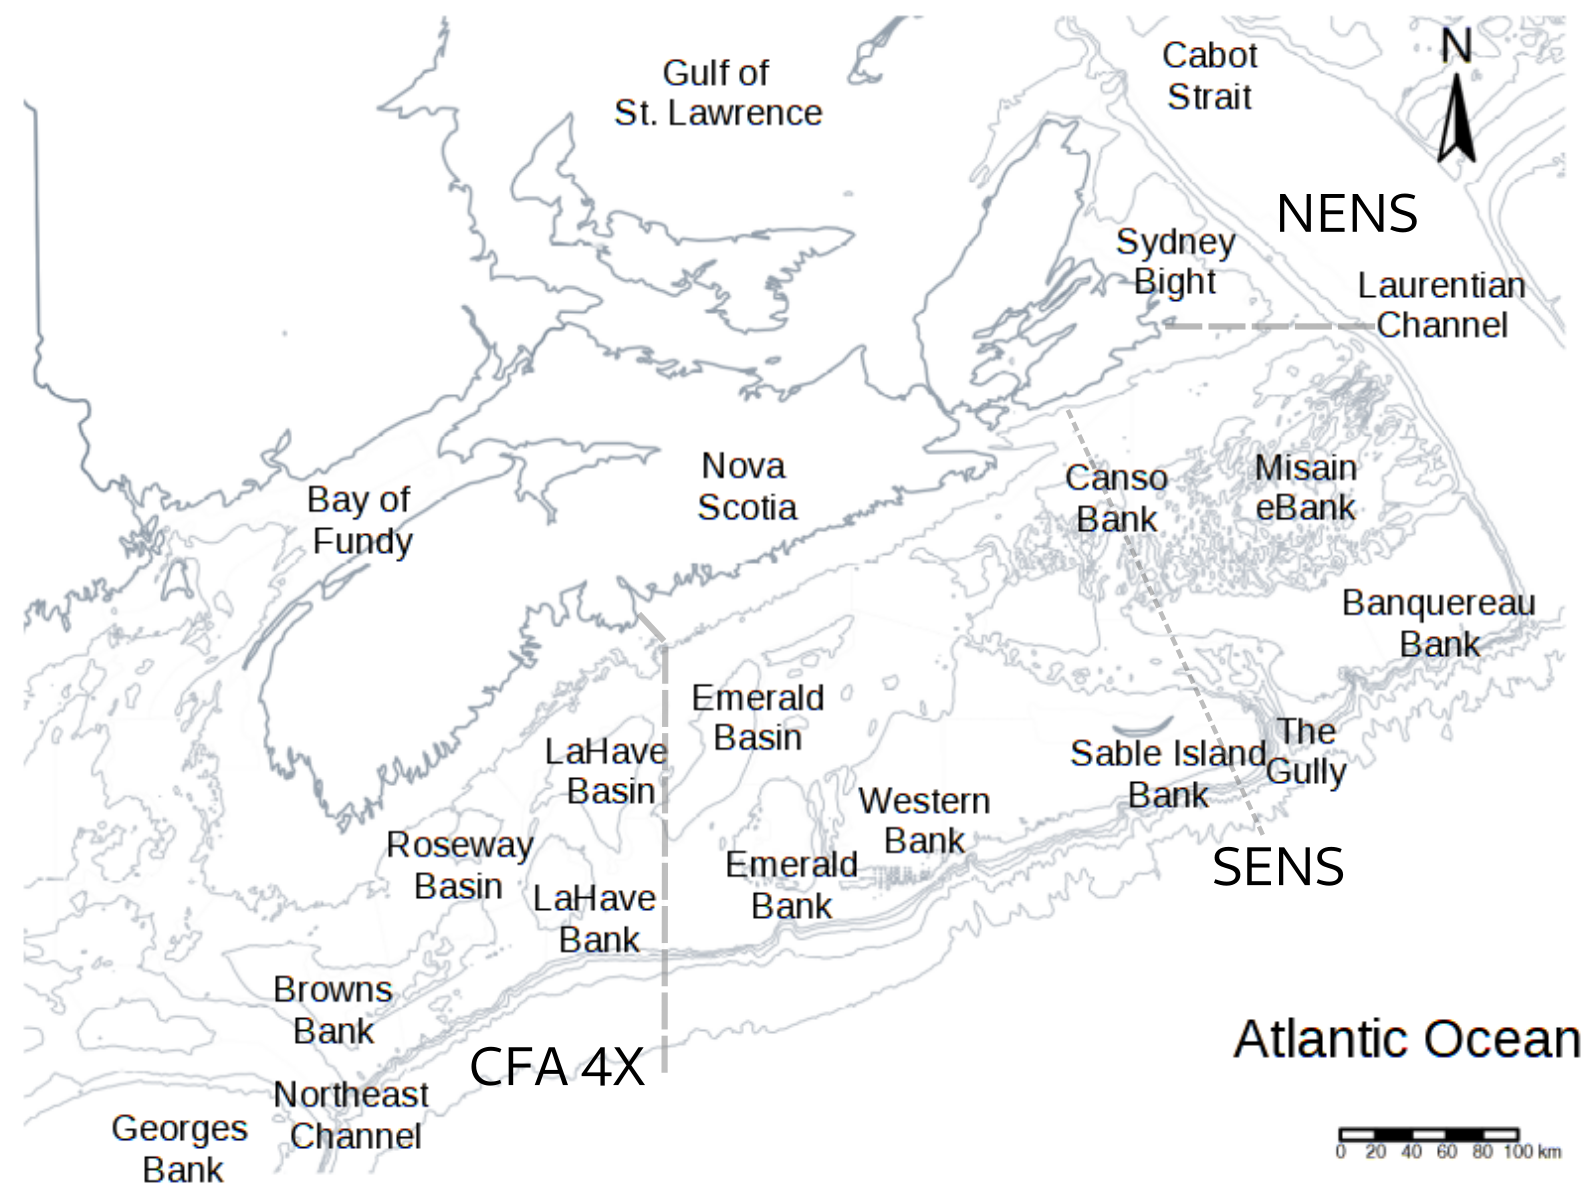
\includegraphics[width=\linewidth]{media/area_map.png}
	\caption{The area of interest in the Scotian Shelf of the
	northwest Atlantic Ocean, Canada. Shown are isobaths
	and some of the major bathymetric features in the area. This area is at
	the confluence of the Gulf Stream from the south and south east along
	the shelf edge, Labrador Current and St. Lawrence outflow from the north
	and north east, as well as a nearshore Nova Scotia current, running from
	the northeast. It is hydro-dynamically complex due to mixing of
	cold, low salinity water from the north with the warm saline water from
	the south. Shown also are the managed Crab Fishing Areas divided
	by thick dashed lines: NENS (North-Eastern Nova Scotia), SENS (South-Eastern Nova Scotia), 
	CFA 4X Crab Fishing Area 4X).}
	\label{fig1}
	\end{figure*}   
	


Unfortunately, characterizing snow crab population dynamics is remarkably difficult (Figure~\ref{fig2})). This is because they are long lived and have a complex life history. Ultimately this translates into large vertical and horizontal shifts in spatial distributions as they grow older (ontogenetic shift in habitat). Functionally, they participate in the pelagic and subsequently benthic ecosystems and associated nutrient and carbon cycles. They also have a narrow range of environmental preferences which coincide with highly variable ocean climates rendering them a challenge to sample. The additional factors of global rapid climate and ecosystem change make this understanding even more difficult. Some of the notable life history features of snow crab that make them so interesting but difficult to model, include: sexual dimorphism with mature males being much larger than mature females; pelagic larval stages and benthic pre-adolescent and adult stages; semi-annual and annual molts depending upon size, age and environmental conditions; terminal molt to maturity; and longevity up to 15 years. They also have a narrow range
of temperature preferences \cite{Foyle_et_al_1989, Sainte-Marie_Lafrance_2002, Kuhn_Choi_2011}. 
They are thought to avoid temperatures above $7^{\circ}C$, as metabolic costs have been shown to exceed metabolic gains
above this temperature in laboratory studies \cite{Foyle_et_al_1989}. Smaller crab and
females also have differences in thermal preferenda \cite{Choi_et_al_2022}. Further,
snow crab are generally observed on soft mud bottoms; with
smaller-sized and molting crabs showing preference for more complex
(boulder, cobble) substrates, presumably as they afford more shelter
\cite{Sainte-Marie_Hazel_1992, Comeau_et_al_1998}.
	
\begin{figure*}
	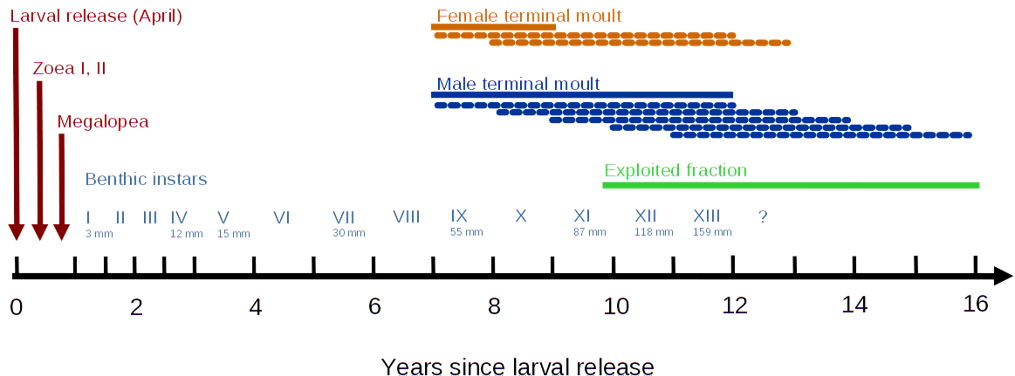
\includegraphics[width=\linewidth]{media/life_history.png}
	\caption{Life history patterns of snow crab and approximate timing
	of the main life history stages since larval release of snow crab and size (measured as
	carapace width; mm) and instar (Roman numerals). Size and timings
	are specific to the area of study and likely vary with regional environmental
	conditions, food availability and genetic variability. Brooding time is variable and is between 1 and two years. Terminal molt to maturity (orange and blue lines) also vary in timing.}
	\label{fig2}
	\end{figure*}   
	 


Snow crab eggs are brooded by their mothers for up to two years,
depending upon ambient temperatures as well as food availability (which
also depends upon temperature as it influences overall system primary
and secondary production) and the health condition and maturity status
of the mother (up to 27 months in primiparous females (first breeding event)
event; and up to 24 months in multiparous females (second and subsequent breeding events) \cite{Sainte-Marie_1993}. More rapid development of eggs, from 12
to 18 months, has been observed in other areas \cite{Elner_Beninger_1995, Webb_et_al_2007}. Over 80\% of the female snow crab on the Scotian Shelf are estimated to follow an
annual cycle, possibly due to extended periods of exposure to warmer
temperatures \cite{Kuhn_Choi_2011}. A primiparous female of approximately~58~mm
carapace width produces between 35,000 to 46,000 eggs, which are
extruded between February and April \cite{Sainte-Marie_1993}. Multiparous females are
thought to be more fecund, with more than 100,000 eggs being produced by
each female. Eggs are hatched from April to June when larvae are
released. This pelagic larval stage lasts for three to five months (Zoea
stages I and II) during which snow crab feed upon zooplankton. Pelagic
stages seem to have highest abundance in October and so may begin
settling in January \cite{Kuhn_Choi_2011}. Thereafter, they settle closer to the
ocean bottom in their Megalopea stage. Very little is known of survival rates
at these early life stages, but they are thought to depend highly
upon temperature \cite{Sainte-Marie_Lafrance_2002}. 

This paper reviews some of the historical attempts at modeling snow crab dynamics and identifies a novel approach that overcomes historical difficulties by incorporating observation error across sex and stage-structure and habitat variability to simultaneously model population dynamics and infer population parameters. We examine its utility and demonstrate the mechanism by which we can make these and more complex models operationally viable through the use of efficient and modular computing that simultaneously models and infers parameters by leveraging \textbf{Julia} programming environment \cite{Bezanson_et_al_2017} and
the supporting \textbf{Turing} library \cite{Ge_et_al_2018} for
Bayesian parameter inference and the \textbf{DifferentialEquations} library \cite{Rackauckas_Nie_2017} for dynamical modeling. This examination is conducted in the Scotian Shelf Ecosystem (Figure~\ref{fig1}) where the variability of ocean climate is known to be high \cite{Choi_et_al_2004, Drinkwater_2005} and where we also have a consistently sampled population since the late 1990s. The principal conclusion of this study is that the novel proposed model is informative and demonstrates utility in understanding snow crab dynamics more coherently and versatility in incorporating ecosystem effects upon habitat viability. It is flexible in approach to permit other ecosystem factors such as classical inter-specific interactions and movement which are planned for future studies.

 
%------------------------------------------------

\section{Methods}

Data collection and subsequent index estimation are described in \cite{Choi_2020, Choi_et_al_2022}. In short, sampling in an unbiased manner under complex hydrodynamic conditions is particularly difficult as the random stratified sampling (i.e., spatial) that is usually adopted to account for such variability, fail to do so due to the large dynamic (i.e.,spatiotemporal) structures operating on scales comparable to the domain. A model-based approach (\emph{Conditional AutoRegressive Spatiotemporal Models}, \textbf{CARSTM}, \url{https://github.com/jae0/carstm}) are used to address the estimation problem. More specifically, biases induced by differential spatiotemporal variability in habitat for differing life stages which upon aggregation across
space, permits an index of abundance comparable across time (years). 
This study focuses upon the indices of abundance derived from this process for the period from 1999 to 2022. Importantly, no survey was conducted in 2020 due to Covid-19 related uncertainties. The index generation method being Bayesian, imputes these estimates, but
variability attached to this year is large. These aggregate timeseries data and supporting \textbf{Julia} models used in this paper are available at: \url{https://github.com/jae0/dynamical_model/tree/master/snowcrab}.

In the area of study, the continental shelf of the northwest Atlantic
Ocean (Figure~\ref{fig2}), snow crab are exposed to high bottom temperature 
variability due to the confluence of a number of oceanic currents: the warm Gulf Stream, the
cold Labrador current, low salinity outflow from the St. Lawrence river
and the cold coastal Nova Scotia current. In this region, snow crab are
generally observed between depths of 50 to 300 m and between
temperatures of $-1$ to $11^{\circ}C$ \cite{Choi_2011}. As the focal area is thermally
complex, their spatial distributions can fluctuate seasonally and
annually. 

There have only been a small number of attempts at modeling the dynamics
of snow crab populations. Being long-lived, sexually dimorphic, deep
water, benthic organisms, usually living far offshore, they are not
easily surveyed. Snow crab have a complex life history that spans
up to 15 years from planktonic to benthic stages. They molt 2 times
a year in the early stages and then approximately annually by instar
5 (about 15 mm carapace width) and can even skip molts when living conditions
are poor. This life history complexity causes complexity in their
dynamics and spatial distributions. Most population assessments approach
abundance estimation as a fishery- or survey-based relative index
of a narrow segment of the population (the fishable component). When
modeled, these empirical estimates of abundance are assumed to be
known without bias.

Further, aging of snow crab is not possible due to a lack of retention
of calcified body parts through molts. This has encouraged adoption
of size-based models \cite{Siddeek_et_al_2009, Cadigan_et_al_2017, Ianelli_et_al_2022},
often with strong and questionable assumptions. For example, \cite{Siddeek_et_al_2009}
assume the male fishable component is the spawning stock biomass,
though of course it is the females that are the reproductive component
and completely unexploited with a shorter life span. Similarly, \cite{Choi_Zisserson_2011} implicitly assumes that the fishable biomass regenerates itself by application
of a biomass dynamics model. Importantly, sex and size-selectivity
of sampling gear are almost always assumed to be a constant or some
smooth monotonic function of body size, and so static across time
and space. These are significant and biologically problematic assumptions.
The problems encountered are fundamental
issues shared with all other attempts at assessment. Specifically, they are the interplay between snow crab life history and behavior; our inability to observe them without bias
due to sampling design being non-random with respects to the environmental
factors controlling their distribution and abundance; and the sampling
machinery (mesh size, trawls that cannot access rugose areas) that
can only observe a small fraction of the population.
 

The \emph{phenomenological} single component model of Verhulst which
was first used to describe Belgium's population growth is well understood
\cite{Verhulst_1845, Bacaër_2011}; see Appendix~\ref{logistic}:

\begin{equation}
	\frac{\mathit{dN}}{\mathit{dt}}_{}=\mathit{rN}{({1-\frac{N}{K}})}.
\end{equation}

It is parameterized by an intrinsic rate of increase ($r$) representing
the maximum exponential rate of increase and carrying capacity ($K$)
the upper threshold. When numerical abundance 
$N\rightarrow0$, the loss term also 
$\frac{N}{K}\rightarrow0$, and so 
$\frac{\mathit{dN}}{\mathit{dt}}_{}\rightarrow\mathit{rN}$. When 
$N\rightarrow K$, then 
$\frac{N}{K}\rightarrow1$ and so the loss rate approaches 
$\mathit{rN}$ and the overall rate of change approaches zero 
${\frac{\mathit{dN}}{\mathit{dt}}_{}\rightarrow0}{}$.
Parenthetically, this can be simplified further by dividing both sides
by $K$ to give: 
${{\frac{\mathit{dN}}{\mathit{dt}}/K}_{}=\mathit{rN}}{{({{1-r}\frac{N}{K}})}/K}.$ By focusing upon 
$n=\frac{N}{K}$ as a non-dimensional number ranging from (0,1), this becomes: ${\frac{\mathit{dn}}{\mathit{dt}}_{}=\mathit{rn}}{({1-n})}$. For parameter estimation/inference, this form is useful as it is simpler and the magnitudes of variables are mostly similar, with the exception of 
$K$. This renders beneficial properties to numerical optimization procedures. 
The sigmoid nature of the equation has rendered it a frequently encountered
model that shows versatility in phenomenologically describing population
dynamics. Its discrete form is particularly common in fisheries settings
\cite{Schaefer_1954, Meyer_Millar_1999} and
has also been used to describe snow crab dynamics in the area of study
\cite{Choi_Zisserson_2011}. The focus is usually upon biomass 
$B$ and its normalized value, ${{b=B}K^{-1}}_{},$ rather than numerical abundance: ${b_{t+1}={b_{t}+\Delta}}b_{t},$ where $\Delta b_{t} = rb_{t}{({1-b_{t}})}-\mathit{Fishing}_{t}K^{-1}.$ Here, $\mathit{Fishing}_{t}$ is scaled by 
$K$ to make it non-dimensional and also in the interval (0,1); it is usually
treated as an external factor (perturbation), measured without error.
Of course, there is usually observation error and/or illegal removals
that will get erroneously absorbed as a biological process; in this case by elevating
the intrinsic rate of increase to compensate for the additional losses.
This will have an effect of creating bias and uncertainty in related
parameters (see below). Note also that the discretization to an annual basis is a significant assumption as the time span is large relative to the processes of most biota.
This has the effect of averaging out sub-annual dynamics. This means
temporal aliasing or discretization errors and censoring are introduced
which ultimately increases process and observation errors (see subannual
dynamics, below).

From this \emph{phenomenological} view, the minimal parameters required
to estimate biological reference points, and the relative distance
a system is from such reference points help delimit the status of
a population \cite{Schaefer_1954, Meyer_Millar_1999}.
Values such as Maximum sustainable yield 
$\left({\mathit{MSY}={\mathit{rK}/4}}\right)$ and the fishing mortality associated with such a yield 
$\left({\mathit{FMSY}={r/2}}\right)$ are commonly used to help define some consistent landmarks of scale
for use as management reference points to guide the implementation
of consistent \emph{Precautionary Approach} for fishery exploitation.

Many approaches exist to estimate these model parameters. Currently,
\emph{Maximum Likelihood} approaches dominate due to their computational
speed. However, it has been the author's experience with this data that they do not
navigate and optimize very high-dimensional parameter spaces reliably,
especially in the delay differential equation models that we explore, below.
This renders their utility in an operational setting, minimally useful.
The related \emph{Maximum A-Posteriori} solutions, where using the
same optimization techniques but with the addition of ``prior-like'' constraints
can result in marginally more stable results, but they still have tremendous
difficulty with high dimensional parameter spaces and the associated numerous local
optima/multiple equilibria.

The operationally most viable approach encountered so far has been
Bayesian inference, where informative priors for these parameters
are explicit and variance propagation of index variables can be accomplished
by using them as priors to respective likelihood error terms, rather than some adhoc nuisance constraint. They facilitate parameter estimates that are stable and credible, given
some latent process and observation models \cite{Meyer_Millar_1999}.
Previously, JAGS (Just Another Gibbs Sampler \cite{Plummer_2003})
and STAN \cite{Stan_2022} were
used to compute the posteriors via MCMC \cite{Choi_Zisserson_2011}.
The latter uses the more efficient NUTS sampler which significantly
speeds up the estimation process of these discrete difference equation
models. Presently, we use \textbf{Julia} programming environment \cite{Bezanson_et_al_2017} and
the supporting \textbf{Turing} library \cite{Ge_et_al_2018} for
parameter inference and the \textbf{DifferentialEquations} library \cite{Rackauckas_Nie_2017} for
modeling delay differential equation models; they demonstrate orders
of magnitude greater efficiency and flexibility to simultaneously model 
and infer parameter values in such problems,
relative to basic MCMC procedures due to use of automatic differentiation
and heavily optimized solution engines.

As a basic point of reference, we use the simplest possible (\emph{phenomenological})
model discretized to an annual basis \cite{Choi_Zisserson_2011}. The latent (real but
unobserved) biomass was assumed to have a \emph{process model error}
that is a recursive Gaussian or Normal distribution ($N$) with a standard deviation $\sigma_{p}$ {(Bolker 2008)} such that:


\begin{equation}
	\label{eq2}
	b_{t+1}\sim N({{{b_{t}+r}b_{t}}{{({1-b_{t}})}-\mathit{Fishin}}g_{t}K^{-1},\sigma_{p}}). 
	\end{equation}

Here, ``$\sim$'' indicates ``distributed as''. Marginally informative priors were assumed: $r\sim N\left({1.0,0.1}\right)$, 
and $K\sim N\left({\kappa,0.1\cdot\kappa}\right)$. The prior mean of the carrying capacity (
$\kappa={\lbrack{5.0,60,1.25}\rbrack}$, in kt, for the North, South, and area 4X (\ref{fig1}), respectively) were based upon historical analyses with other analytical procedures, namely Geostatistical Kriging with External Drift and Generalized Additive Models \cite{Choi_et_al_2005b, Choi_2011}. 

It is further assumed that the real unobservable (latent) process $b$ is sampled with error (observation standard deviation 
$\sigma_{o}$ ). The \emph{observation error model} in most fishery applications is a simple
multiplicative factor, often referred to as a ``catchability'' coefficient 
$q$. In this case we assume that: $q\sim N\left({1.0,0.1}\right)$, and so the \emph{observation error model} becomes:


\begin{equation}
	\label{eq3}
	Y_{t}\sim N({q\mathit{Kb}_{t},\sigma_{o}}). 
	\end{equation}
 
This means that the observed biomass indices $Y$ are some constant fraction of the true abundance 
$b_{t},$ across all sampling time (years, season) and locations. The recursive logistic process model (eq.~\ref{eq2}) in tandem with the observation model (eq.\ref{eq3}), we will refer to it as, ``\emph{Model 1}''.
	
\begin{figure*}
	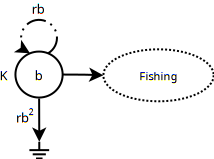
\includegraphics[width=4.5 cm]{media/logistic_diagram.png}
	\caption{A graphical representation of \emph{Model 1} (simple logistic;
	eq. 1). Here, ${b=B}K^{-1}$ is a non-dimensional number that 
	ranges from (0, 1) that represents
	the biomass $B$ after being scaled to $K$. The loop $\mathit{rb}$
	identifies the growth rate and the loss term $rb^{2}$ identifies the
	quadratic increase in ``mortality'' as $b\rightarrow1$. Fishing is 
	also scaled to $K$, such that: 
	${\frac{\mathit{db}}{\mathit{dt}}_{}=\mathit{rb}}-\mathit{rb}\cdot{{b-f}={\mathit{birth}-\mathit{death}-\mathit{fishing}}}$; and total mortality = death + fishing.} \label{fig3}
	\end{figure*}   


From the graphical representation of the processes of \emph{Model 1} (Figure
4), one can immediately see that there is no input term from outside
of the system: it is a simple \emph{phenomenological} self-loop model
with two outputs (death and fishing). The term 
$\mathit{rb}$ can be referred to as the (net) ``birth process'' \cite{Gillespie_1992, Qian_Bishop_2010, Albert_2016},
and represents a first order processes that increases 
$b$ (via birth, growth, enhanced survival, improved food availability,
immigration, strong year class strength, etc.), through the single
(static) parameter $r$. The mechanism is not identified and is 
implied to be some internal
recycling of b. In reality, there are biological mechanisms involved
and associated parameters that are not-static and non-stationary (in
first and second order; across time and space). Growth in biomass
or increase in numbers is seasonal and pulsed, due to the molting
process and body mass increases, that progress at variable rates depending
upon time of year and environmental variability. Across years, there
are strong and weak year classes due to match-mismatch type processes
\cite{Cushing_1969, Durant_et_al_2007},
and so also pulsed. These simple models cannot address these more
realistic dynamics and so we obtain instead, an average state, with
poor resolution of peaks and troughs and so parameter estimates that
are likely to be in error.

The strength of \emph{Model 1} is simplicity; but this simplicity
is also a weakness. As the biomass dynamics model is phenomenological;
it is heuristic, without mechanism. For example, fishable biomass
``creates'' fishable biomass at a maximum exponential rate (r) to
a limit of K. In reality, fishable biomass being mature male snow
crab, does not produce more mature male snow crab; instead, it is
the female mature population that creates the eggs and broods them
to larvae, some fraction of which eventually mature into the fishable
component. The dynamics and longevity of these females are very different
from those of the males, often showing unbalanced sex ratios and differential
utilization of habitat \cite{Choi_et_al_2022}.
The rate of increase in biomass is not a simple exponential rate;
instead, a certain number of fishable crab die from various causes
(predation, disease, competitive fighting), a certain number of recruits
terminally molt to a size in the fishable range to increase their
numbers, they grow in weight as they eat, some fraction move in and
out of a given area, and some are fished; these rates are not constant
in time nor space and there are many lags in time. Fundamentally it
is a numerical process. So \emph{Model 1} from the perspective of ``biomass
dynamics'' is less than satisfactory in terms of biological realism.
However, in the heuristic perspective, it implies that the biomass
in one year is related to the biomass in the previous year within
some constraints, constraints that are only diffusely/indirectly related
to the ``real'' mechanistic processes represented by individual-individual
interactions. As such, they can be seen as a temporal autoregressive
model.

These constraints unfortunately result in a model that is sometimes
not responsive enough to large fluctuations in dynamics caused by
intrinsic and/or extrinsic factors. For example, due to the pulse-like
dynamics observed since the late 1990s, no recruits entered fishable
components for a number of years, even though their abundance was
low \cite{Choi_2011}.
\emph{Model 1} expected recruitment simply because biomass was low. This
was an erroneous expectation given the low numbers of pre-recruits
that lasted for an extended period of time, nor the extremes of bottom
temperature and associated shifts in their distributions nor the increase
in abundance of predators that followed which reduced the further
the strength of that recruitment. \emph{Model 1} is too simple to express
the expectations of such highly nonlinear pulse-like dynamics and
interactions with environment and predators. In another example, there
was an extreme warming event in 2021 that significantly altered and
constricted the spatial distribution of snow crab \cite{Choi_et_al_2022}.
Again a simple model such as \emph{Model 1}, with static expectations of
environmental conditions are not able to account for such effects.

In an attempt to \emph{begin} addressing these issues, we entertain
\emph{Model 2} (Figure~\ref{fig4}) which resolves some size groups, sex and
maturity and permits time-varying viable habitat area. \emph{Model 2} is,
therefore, an intermediately complex, marginally more structural and
mechanistic (\emph{ontological}) model relative to \emph{Model 1} (Appendix~\ref{continuum}).

\begin{figure*}
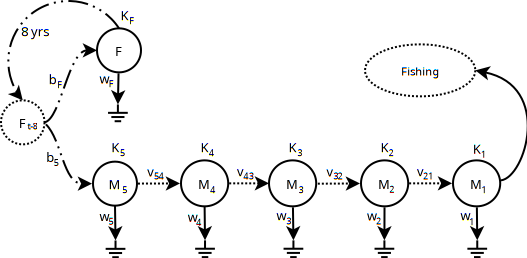
\includegraphics[width=10.5 cm]{media/delay_differential_diagram.png}
\caption{Graphical structure of the six-component \emph{Model 2} of snow
crab with associated numerical flows. 
$F$ indicates mature females, determined from size range and morphometric
maturity. Associated with each component is a carrying capacity ($K_{i}$), and a death rate 
$w_{i},$ and molt rates $v_{\mathit{ij}}$ ; and birth/survival rates 
$b_{i}$. $F_{t-8}$ is the state of mature females $F$ from 8 years prior. Fishing is considered an external, deterministic sink imposed by external factors.} 
\label{fig4}
\end{figure*}   
	


There is approximately an 8+ year period that is required for females
$F_{t-8}$ to produce the next generation of instar 9 females and males, denoted
by $F_{t}$ and $M_{5,t}$, respectively. They represent crabs in the range of approximately
40 to 60 mm carapace width. The ``birth'' rates represent a combination of egg
production and larval survival to instar 9+. If the population is
stable, ``birth'' rates are expected to be similar in magnitude
to overall death rates. Note that ``stage'' is defined based upon
size-sex-morphometric traits and so misclassification is likely. The
error in such knife-edge stage determinations can be substantial if
growth and maturity schedules vary significantly. It is assumed, here,
that in the aggregate, this has been stable in the survey record (1999
to 2021). This may of course be incorrect if persistent size/stage/age
related mortality occurs due to exploitation/predation patterns and/or
directional environmental change such as climate warming or food availability
shifts.

Some fraction of instar 9 males transition to instar 10 ($M_{4}$), and then 11 ($M_{3}$) to 12 ($M_{2}$) and 13+ ($M_{1}$); each transition rate parameterized by 
$v$, with numeric indices identifying the instar pairs. Due to the knife
edge-cut of stages, there will be misclassification issues which will
be absorbed by these transition rates. For example, a small fraction
of instar 11 crab ($M_{3}$) will be large enough to be considered a fishable size (\textgreater95mm carapace width); but most will molt into instar 12 ($M_{2}$); this would result in a reduced molt transition rate. 
$M_{2}$ will represent a composite group of most crab that have entered fishable
size but are still immature. Some fraction of this group will mature
into the fishable component in the next year; the fractional nature
will result in a smaller molt transition rate. Others will continue
to molt to instar 13 and higher; for our purposes, all morphologically
mature males of fishable size will be considered 
$M_{1}$ and so it represents a range of different ages. This is especially
the case as terminally molted crab can live for up to another 5 years;
this aggregation will effectively decrease mortality rate of the group.

Survey sampling and estimation of instar 9 to 13+ (40 mm to 130+ mm
carapace width) is reasonably informative. Earlier instars tend to have more divergent
habitat preferences relative to those of the fishable component and
are also known to be poorly/erratically sampled due to their being
small enough to be significantly affected by sampling mesh size. This
is because the snow crab surveys are primarily optimized for sampling
the fishable component (\textgreater{} 95 mm carapace width), both in terms
of mesh size and choices of sampling location. The utility of these
additional compartments is that they also permit more stable parameter
estimation and forward projections that are biologically more reasonable
(mechanistic). The challenge is to keep track of much more information
due to the increased realism and computational limits. Each state
variable $U={({M_{1},M_{2},M_{3},M_{4},M_{5},F})}$, is scaled by their respective carrying capacity $K_{i}$, such that they are non-dimensional numbers: 
${u_{i}={({U_{1}K_{1}^{-1},U_{2}K_{2}^{-1},U_{3}K_{3}^{-1},U_{4}K_{4}^{-1},U_{5}K_{5}^{-1},U_{6}K_{6}^{-1}})}}.$ Thus, for example, in the molt transition process from 
$i=2$ to $j=1$, the instantaneous rate is: \\

$v_{21}u_{2,{t-1}}{a_{21}=v_{21}}{({U_{2,{t-1}}K_{2}^{-1}})}K_{2}K_{1}^{-1} = v_{21}U_{2,{t-1}}K_{1}^{-1}$. \\

The multiplier ${a_{21}=K_{2}}K_{1}^{-1}$ is required to convert normalized density of category 2 to that of category 1 via the ratio of the respective normalizing constants,
$K_{i}.$ As with \emph{Model 1}, first order birth/survival rates 
$b_{i}$ are assumed: ${\beta_{i}=b_{i}}u_{i}.$ 

So far, most of the core model has been the same as \emph{Model 1}, only
applied to more components with some appropriate time lags. Where
\emph{Model 2} diverges from \emph{Model 1} is by decomposing mortality into two
components: the first component is a simple background mortality parameterized
as a first order decay ${({\omega_{i}u_{i,t}})};$ the second component is
mortality associated with fluctuations of
viable habitat, parameterized as in the logistic equation as in \emph{Model 1} as a second
order process $\psi_{i}\frac{U_{i,t}}{K_{i,t}H_{\mathit{it}}}\cdot U_{i,t}$. Note the congruence with the $r\frac{N}{K}\cdot N$ loss term of \emph{Model 1} (see Fig. 4, eq. 1), such that upon normalization
to $u$, we obtain: \\

${w_{i,t}=\omega_{i}}{u_{i,t}+\psi_{i}}\frac{{u}_{i,t}}{H_{i,t}}\cdot{u}_{i,t}.$ \\

Here, ${H={V/\mathit{\max}}}{(V)},$ represents the viable habitat surface area 
$V{}$ normalized to a maximum value of 1, where the maximum is defined in
the reference/focal time period. This modifies the carrying capacity
proportionately and so  $\mathit{KH}$ can be seen as the ``effective carrying capacity'',
adjusting for viable habitat fluctuations. The assumption here is that when viable
habitat area declines by some fraction $H$, so too does the effective carrying capacity, proportionately.

The inclusion of predator-prey and other ecological processes are
therefore straightforward extensions as additional terms in this type
of model formalism are well understood in the literature \cite{Lotka_1920, Bertalanffy_1950, Pianka_1970, Wangersky_1978}. Such extensions are planned for future research and evaluation.

The full set of delay differential equations are, therefore:
\begin{align*} 
\frac{\mathrm{d} u_{1}}{\mathrm{d} t} &= v_{21}u_{2,{t-1}}a_{21}-w_{1,t}-\mathit{Landings}_{t}K_{1,t}^{-1} \\ 
\frac{\mathrm{d} u_{2}}{\mathrm{d} t} &= v_{32}u_{3,{t-1}}a_{32}-v_{21}u_{2,t-1}-w_{2,t} \\
\frac{\mathrm{d} u_{3}}{\mathrm{d} t} &= v_{43}u_{4,t-1}a_{43}-v_{32}u_{3,t-1}-w_{3,t} \\
\frac{\mathrm{d} u_{4}}{\mathrm{d} t} &= v_{54}u_{5,t-1}a_{54}-v_{43}u_{4,t-1}-w_{4,t} \\
\frac{\mathrm{d} u_{5}}{\mathrm{d} t} &= b_{5}u_{6,t-8}a_{56}-v_{54}u_{5,t-1}-w_{5,t} \\
\frac{\mathrm{d} u_{6}}{\mathrm{d} t} &= b_{6}u_{6,t-8}-w_{6,t}.
\end{align*}  


\emph{Model 2} is, therefore, a slightly more mechanistic (structured) extension of \emph{Model 1} that brings to bear additional information available about the abundance
of other size and sex classes and transition rates between them, and
mortality rates that depend upon variations of numerical density in viable habitat surface area. 

Fishery landings were converted to number based upon annual average
weight of the fishable component estimated from surveys and discretized
to a two week time step within each year. The latter was to avoid
strong discontinuities which facilitates differential equation modeling
and parameter inference. Survey-based indices of numerical abundance
were estimated using a Hurdle process, where probability of observation
and the numerical abundance of positive-valued observations were modeled
as an extension of small-area analysis (Conditional AutoRegressive
Models in space and time; see methods in \cite{Choi_et_al_2022, Choi_2022}.
Modeled average weights, also analyzed using the same small-area space-time
analyses were used to convert numbers back to biomass to make comparisons
with \emph{Model 1}.

In \emph{Model 1}, the meaning of 
$q$ is clear: a survey catches only some (fixed) fraction of the true
abundance. This is a reasonable first approximation. However, what
is implied is: first, this fraction is unchanging, applying equally
in high abundance and low abundance years and areas, whether they
are in the mating or molting season or not. Ignored are issues such
as differential net saturation, aggregation behavior, even when bottom
temperatures can force aggregation and dispersal away from or into
other areas. The second issue implied by 
$q$ is that when a survey fails to capture snow crab, that there truly
is no snow crab in the area: an observation of zero is a true zero.
\textbf{\emph{This is clearly false}}. Visual observation of trawl operation
through video monitoring have shown that crabs are missed: when they
are in a slight depression, when they are close to protruding rocks
or on bedrock, when bottom topography is complex or simply by the
gear jumping off of the bottom due to tidal currents. That is, sampling
gear is biased. Furthermore, it is not just sampling gear that is
problematic. Survey design is biased: in design, each areal unit is
expected to be homogeneous in space AND time. External factors being
factored out such as bottom temperatures, food availability and predation,
aggregation behavior are not homogeneous, no matter how well designed
a sampling design may be. Further, there is the notion of \emph{trawlable
bottom}: some areas cannot be sampled without tearing or losing
nets. These areas are of course not sampled and only habitats that
are easier to sample will be used and consequently, over represented.
Though allocation may be \emph{random} in design and theory, in application,
it is at best, \emph{almost random} and depending upon bottom type,
usually biased.

As such, the observation model is also more complex in \emph{Model 2}. The
assumption of zero values in survey abundance indicating a true zero
is a very strong assumption. This is especially tenuous when it is
known that surveys sample many size ranges very poorly. The observation
model of \emph{Model 2} is, therefore, a simple linear regression. Of course,
higher order terms and other covariates can and should enter into
the observation model to account for potential survey and behavior
induced bias. In this paper, this is mostly accomplished via the statistical
abundance index model \cite{Choi_et_al_2022}. Some additional freedom is given in the observation model in that the prior for the intercept term 
$c_{i}$ was informed by 
$\mu_{i}$, the fraction of the minimum observed value relative to the maximum
value.

$m_i \sim N(1.0, 0.1)$,

$c_i \sim N(\mu_i, 0.1)$, and

$y_{\mathit{ti}} \sim N(\mu_i n_{\mathit{ti}} + c_i, \sigma_{ti})$.
Here, ${y_{\mathit{ti}}={Y_{\mathit{ti}}/\mathit{\max}}}{(Y_{i})},$ 
constrains abundance to the interval (0, 1) and helps to confer better
numerical properties (faster and more stable optimization, integration)
in that variables are of similar magnitudes. Additionally, the variability of the observations was propagated into
\emph{Model 2} by assuming that the coefficient of variation of observations
were modal estimates of the observation model using a Lognormal (LN)
prior with a mode of log(CV) specific to each component $i$ and survey
time $t$ and a SD of 0.25 ($\approx 128\%$ error on the normal scale):

$\sigma_{ti} \sim \mathrm{LN}(\log(\mathrm{CV}_{ti}), 0.25)$. 
This works as $y_{\mathit{ti}}$ are already normalized to (0,1). 
The other priors used for the \emph{Model 2} are also informative based upon
expected biological constraints and some very wide distributions for
the variance components to provide well mixed posterior samples as
determined by Effective Sample Size (given autocorrelation in samples
within chains) and \emph{Rhat} (convergence criterion across chains):

$K\sim\mathrm{LN}\left(\log(\kappa),0.25 \right)$,

$b\sim\mathrm{LN}\left(\log(1),0.5 \right)$,

$d\sim\mathrm{LN}\left(\log(0.22),0.25 \right)$,

$\psi\sim\mathrm{LN}\left(\log(0.49),0.5 \right)$, and

${v\sim\mathrm{LN}\left(\log(1.46),0.5 \right)}.$ 

Fixed reference points analogous to the concepts of MSY and FMSY are
not readily identifiable in \emph{Model 2} as ``production'' is now dependent
upon multiple system components each of which have externally imposed
effective habitat viability trends and related natural and fishing
mortalities (perturbations). It is, however, possible to compute a
related concept, which we will call the \emph{fisheries footprint};
it is computed as the difference in trajectories between the system
state estimated for the fishable component with and without fishing.
The biological parameters are estimated under conditions of fishing
activity. In the absence of fishing, these parameters may be expected
to be different, especially when fishing activity is extreme. In some
cases, maturity and growth schedules can shift \cite{Zwanenburg_et_al_2002, Choi_et_al_2004, Choi_et_al_2005a}. The assumption here is that extreme fishing activity has not occurred
with sufficient pressure nor time to generate phenotypic or genotypic
change. The difference in predicted trajectories between the fished
and unfished conditions, therefore, provides a crude, first order
estimate of the impact of fishing, without assumptions beyond that
the model reasonably approximates reality. This fisheries footprint is
placed on a relative scale from 0 to 1, by normalizing with the expected
unfished abundance. As such, the \emph{fisheries footprint} identifies
the fraction of potential biomass that was reduced by fishery exploitation.

 

%------------------------------------------------

\section{Results and Discussion}

Estimates of abundance (biomass) of the exploited component are shown for each region for each model
in Figure~\ref{fig5_predictions}. In NENS, the discrete \emph{Model 1} showed two troughs in (pre-fishery) abundance in 2005 and 2017. The surveyed index after adjustment for
the observation model tends to be lower relative to the pre-fishery
abundance, which is consistent with the removal of biomass during
the fishing season. The exception to this pattern was in late
2013 and 2019 when strong recruitment was also observed. \emph{Model 2} shows
a similar pattern of fall fishable biomass, though with a reduced
magnitude. The post 2019 period showed significant divergence relative
to the survey index and especially in 2020 when no surveys were completed
due to Covid-19 related disruptions. SENS also demonstrated a similar
periodicity to NENS in both models (Figure~\ref{fig5_predictions}). \emph{Model 2} suggests a
dampened time series, attributable to the dynamics of the recruitment
being estimated to be very smooth (Figure~\ref{fig6_m2f}). In CFA 4X, \emph{Model 1}
suggests an important decline following a peak in 2010. \emph{Model 2} suggests
a similar trajectory, though one that is much more variable. This
area is subject to crab movement from the adjoining area as well as
spatial aggregation due to extreme temperature conditions, elevated
mortality from other predators and disease. \emph{Model 2} also suggests
overall abundance that is much lower than the very optimistic expectations
of \emph{Model 1}.

 
\begin{figure*}
	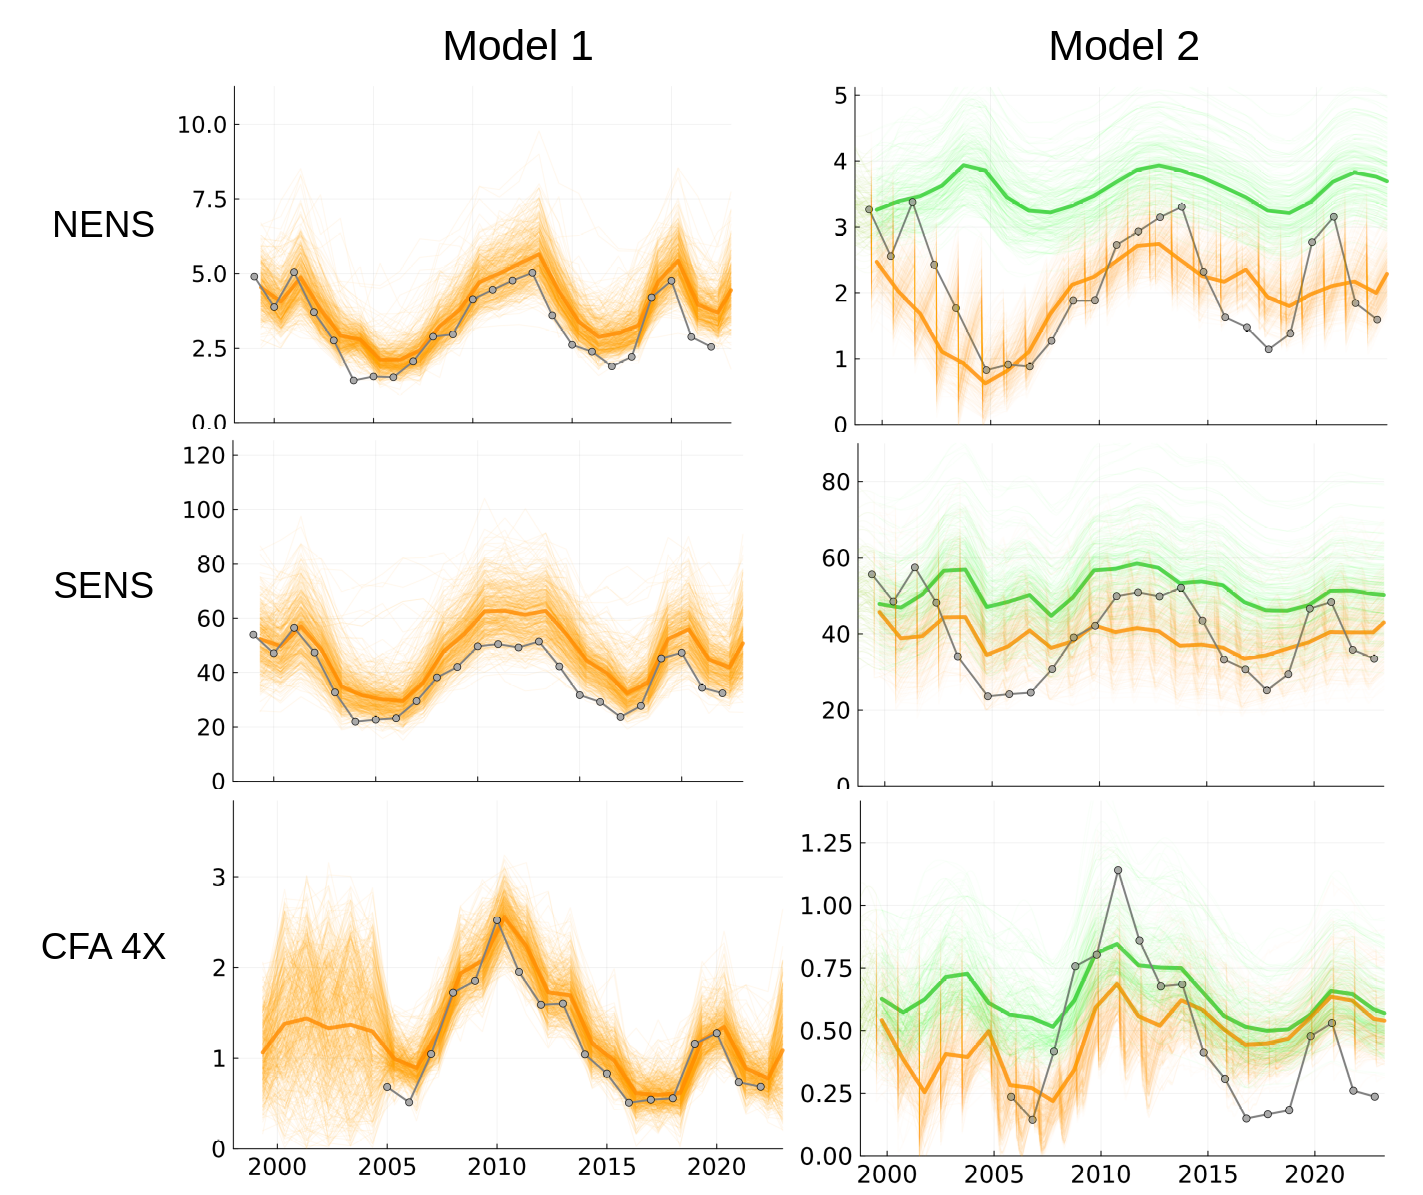
\includegraphics[width=\linewidth]{media/predictions.png}
	\caption{Posterior median biomass (dark orange) for each area of
	study and model. Posterior realizations of dynamics are shown
	to demonstrate variability of solutions. For \emph{Model 1} (left), \emph{pre-fishery}
	posterior estimates of fishable biomass are shown. For \emph{Model 2}, the posterior estimates
	of fishable biomass are shown in orange. Overlaid (gray) in both are
	survey abundance estimates (\emph{post-fishery}, except prior to 2004) after
	correction for their respective observation models. Overlaid in green
	are posterior samples of abundance trajectories expected had there
	been no fisheries exploitation (green); and dark green identifies their means.}
	\label{fig5_predictions}
	\end{figure*}    
 


It is important to note that \emph{Model 1} will project an increase in abundance,
even if recruitment does not exist. It will only project a decline
if abundance is above carrying capacity. This structural expectation
is of course unrealistic. \emph{Model 2}, which accounts for recruitment,
navigates this problem a little more sensibly as increase can only occur if recruitment exceed mortality. For example, it projects for 4X,
a decline, even in the absence of fishing. In SENS, abundance is projected
to increase slightly in the absence of fishing. Only NENS was projected
to have a rapid increase in abundance (Figure~\ref{fig5_predictions}).

Another observation is that abundance may be overestimated by \emph{Model
1}. For example, in 4X where we have supporting information of very
high natural mortality rates associated with predation and environmental
variability, through the loss of strong year classes, abundance estimates
are extremely optimistic. The same issues also exist for N-ENS, where
strong adolescent crab year classes seem to disappear at a rate faster
than might be expected, possibly due to predation. By extension, S-ENS
also likely exhibits overly optimistic time trends, given the very
strong year classes diminishing rapidly before entry into the fishable
component. As a result of this potential overestimation of abundance,
fishing mortality estimates by \emph{Model 1} may in fact be overly low.
\emph{Model 2}'s solutions seem more reasonable given the supporting contextual information
known of the different areas. The overall relative shapes of abundance
and fishing mortality are, however, similar (Figure~\ref{fig7}).

   
\begin{figure*}
    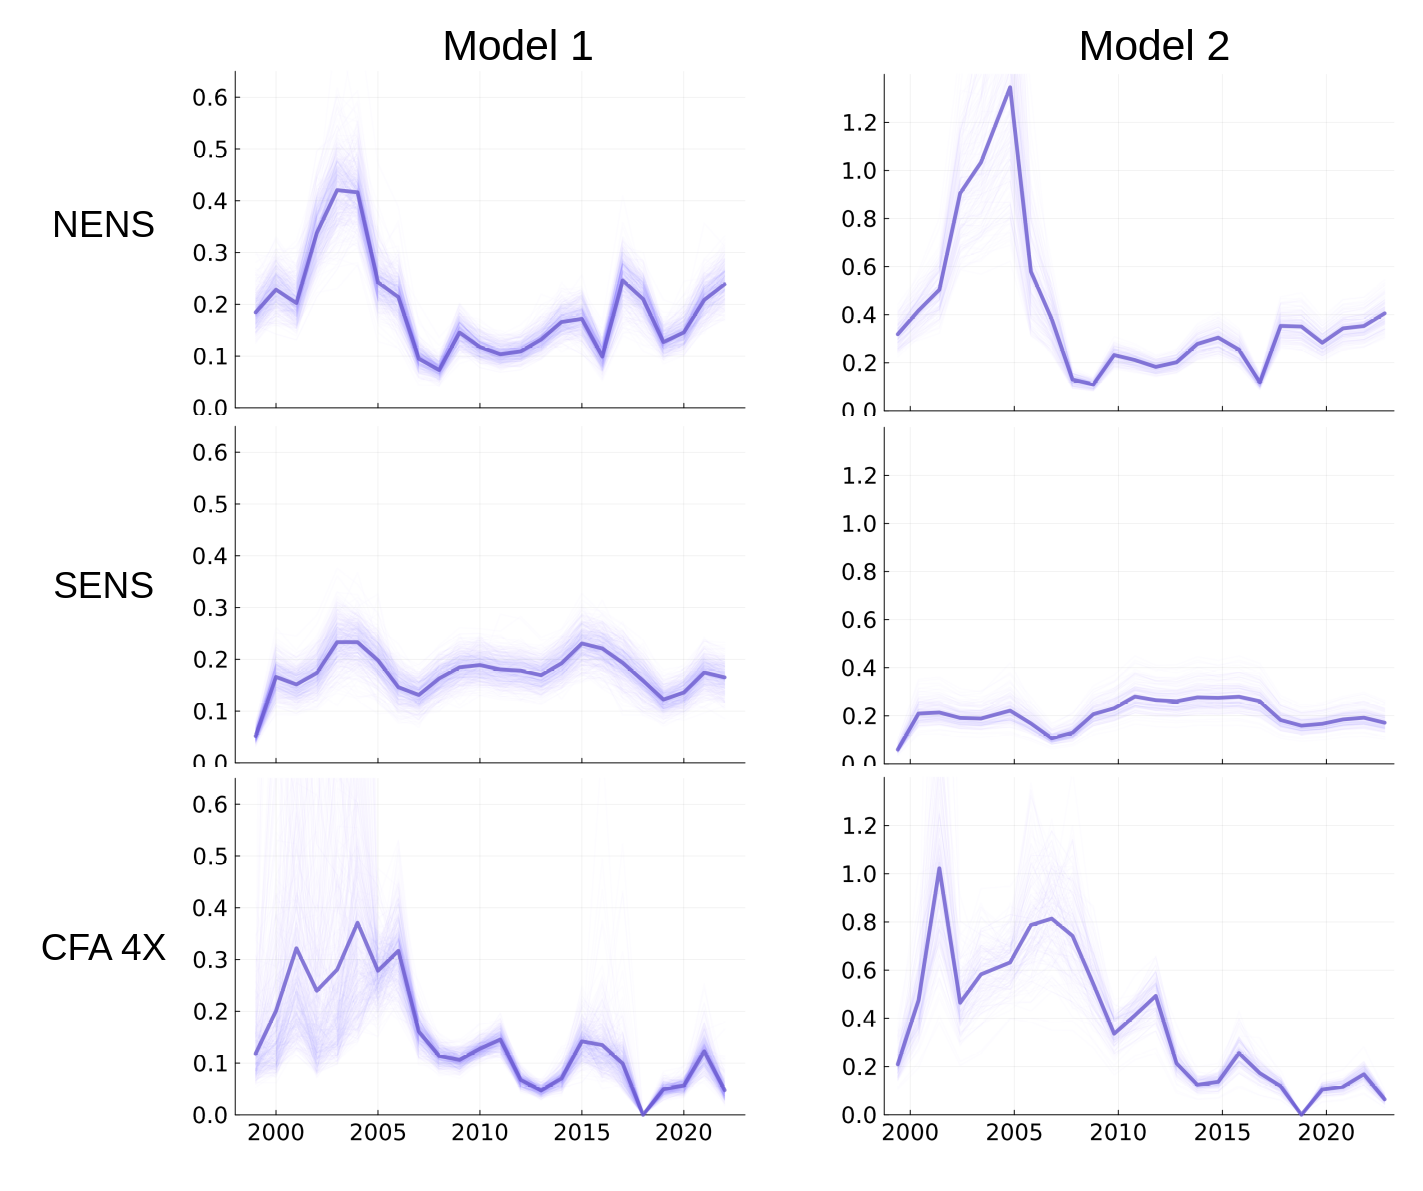
\includegraphics[width=\linewidth]{media/fishing_mortality.png}
    \caption{Instantaneous fishing mortality estimated from \emph{Model 1}
    and 2 across time. The overall patterns of fishing mortality are similar
    across models. However, the overall magnitudes are much higher in
    \emph{Model 2}. Fishing in 4X was closed in 2018 due to low abundance estimates
    and warm environmental conditions.}
	\label{fig7}
    \end{figure*}   


	The continuous form of \emph{Model 2} also permits us to infer the subannual
	dynamics of the snow crab. The saw tooth pattern of abundance (Figure~\ref{fig5_predictions}) suggests that during the fishing season, the rate of exploitation
	far surpasses the slower rate of growth of the fishable component.
	It also identifies how important temporal aliasing might be if observations
	of landings or survey sample times are not properly accounted.
	The fishery footprint across the different areas (Figure~\ref{fig8}) indicates
	that they are very similar to fishing mortality in overall form (as
	they should be, as the numerator, catch are the same). The former
	is on a scale that is the same as abundance and so simpler to understand
	than the exponential scale of an instantaneous rate. \emph{Fishery
	footprint} also has a reasonably direct relationship to a question
	that is often asked in applied situations: \emph{How much of an effect
	is fishing activity having?} In the case of the areas studied, the
	fishery footprint has declined to conservative and manageable levels
	since the mid-2000's. SENS, in particular, has been consistently sustainable
	in the historical record. In the presence of strong environmental
	variability, it will be necessary to continue to maintain a small
	fisheries footprint such that the species does not undergo extreme
	changes in abundance as has been the case for many collapsing fisheries, such as Atlantic cod. This is especially the case as heavy exploitation in the long-term can result in reduced reproductive success of females; loss of dominance by invasion of habitat by competitors and even genetic/phenotypic selection for reduced size at maturity \cite{Comeau_Conan_1992, Choi_2011}.
	 
	 
	\begin{figure*}
		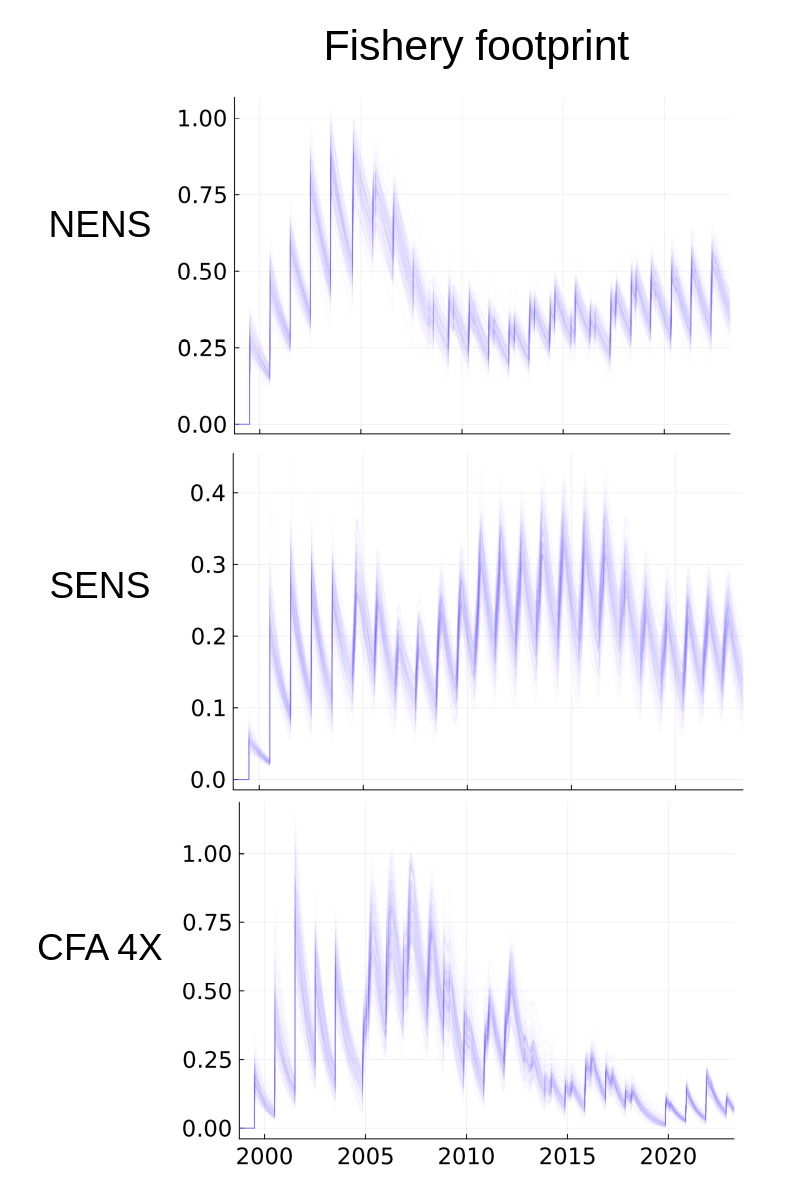
\includegraphics[width=12cm]{media/footprint.png}
		\caption{Posterior realizations of Fisheries footprint for
		each area of study derived from \emph{Model 2}.}
		\label{fig8}
		\end{figure*} 

	The first ever estimate of potential recruitment ($M_{2}$) and mature female abundance ($F$) for the area in focus are shown in Figure~(\ref{fig6_m2f}). It shows that \emph{Model 2} has difficulty tracking these components.
	However, peaks and troughs are identified and they seem to be coherent
	across areas. The lack of concordance with the observations suggest
	that other, as yet unmodeled processes likely need to be better accounted.
	The most likely missing processes include movement (inshore-offshore,
	shallow-deep) as well as predation, as the areas of study are not
	\emph{well mixed} and show spatiotemporal structure and increases in the relative abundance of predators such as Atlantic Halibut. Smaller areal units might be better than the three large areas we used in this
	study to be able to discriminate or at least account for some of these latter heterogenous processes.
	
	
\begin{figure*}
	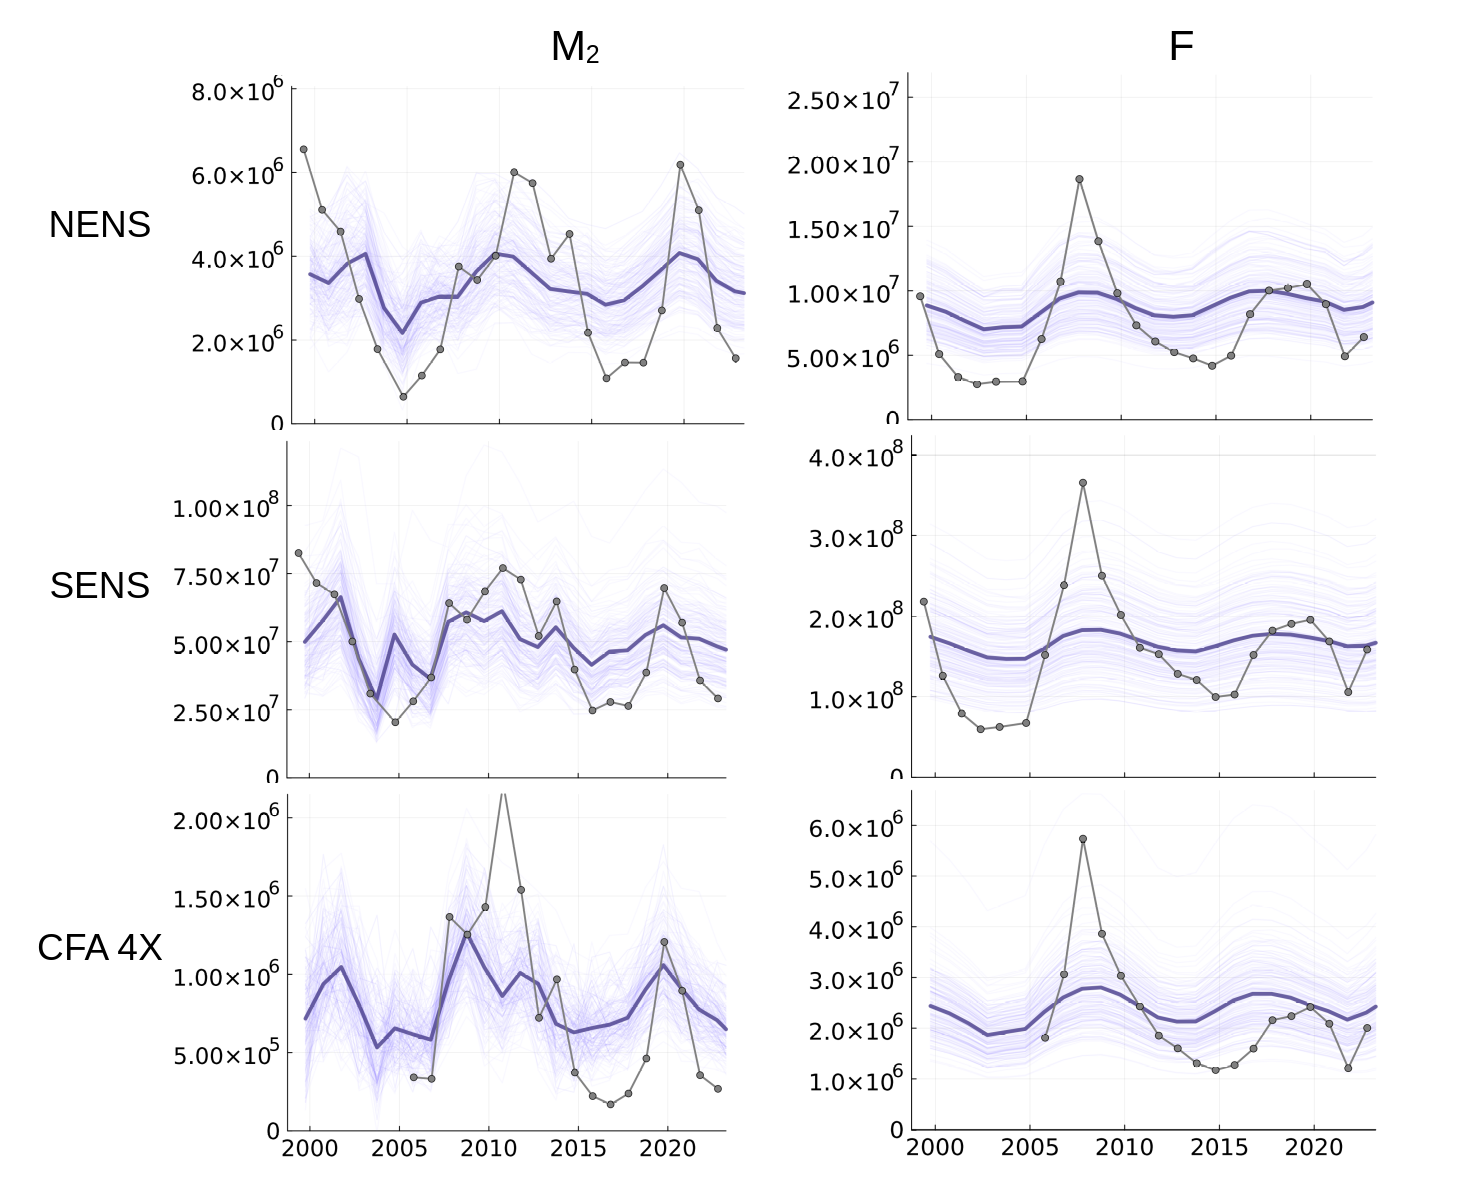
\includegraphics[width=\linewidth]{media/m2_fem.png}
	\caption{\emph{Model 2}posterior numerical abundance for $M_{2}$ (recruits) and 
	$F$ (mature female). Overlaid (gray) are survey abundance estimates (post-fishery,
	except prior to 2004) after correction for observation models.}
	\label{fig6_m2f}
	\end{figure*}   

	  
	  
%------------------------------------------------

\section{Conclusion}

In studies of exploited marine animal populations, most models focus
upon age structure \cite{Quinn_2003}.
Most also tend to be temporally discrete (annual) difference equation approximations. This is largely due to the annual cycle in temperate regions of exploitation,
and data assimilation, survey and assessment cycles and historically
due to limitations to computational capacity. With such discretizations,
come various approximations and assumptions and ultimately potential
error or bias from temporal (and spatial) aliasing. Space is treated
as an externality or more usually, completely ignored, though of course,
advection-diffusion differential equation models are readily formulated.

The continuous approach that we developed in this study addresses
mechanisms in a structured manner. The additional model complexity
succeeds in providing a similar and perhaps more reasonable understanding
of snow crab population dynamics than the classical biomass dynamics
model. It also permits a promising way forward towards describing
the footprint of a fishery measured relative to potential abundance
in the absence of fishing. It also identifies that there are difficulties
that need to be addressed: most notably the \emph{non-well-mixed} nature
of the areas studied show spatial and temporal structures that require
further parameterization and development.


% This statement requires citation \cite{Smith:2023qr}. This statement requires multiple citations \cite{Smith:2023qr, Smith:2024jd}. This statement contains an in-text citation, for directly referring to a citation like so: \textcite{Smith:2024jd}.
 
%----------------------------------------------------------------------------------------
%	 REFERENCES
%----------------------------------------------------------------------------------------
\printbibliography % Output the bibliography

 

  
%%%%%%%%%%%%%%%%%%%%%%%%%%%%%%%%%%%%%%%%%%
%% optional
%\supplementary{The following supporting information can be downloaded at:  \linksupplementary{s1}, Figure S1: title; Table S1: title; Video S1: title.}

% Only for journal Methods and Protocols:
% If you wish to submit a video article, please do so with any other supplementary material.
% \supplementary{The following supporting information can be downloaded at: \linksupplementary{s1}, Figure S1: title; Table S1: title; Video S1: title. A supporting video article is available at doi: link.}

% Only for journal Hardware:
% If you wish to submit a video article, please do so with any other supplementary material.
% \supplementary{The following supporting information can be downloaded at: \linksupplementary{s1}, Figure S1: title; Table S1: title; Video S1: title.\vspace{6pt}\\
%\begin{tabularx}{\textwidth}{lll}
%\toprule
%\textbf{Name} & \textbf{Type} & \textbf{Description} \\
%\midrule
%S1 & Python script (.py) & Script of python source code used in XX \\
%S2 & Text (.txt) & Script of modelling code used to make Figure X \\
%S3 & Text (.txt) & Raw data from experiment X \\
%S4 & Video (.mp4) & Video demonstrating the hardware in use \\
%... &... &... \\
%\bottomrule
%\end{tabularx}
%}

%%%%%%%%%%%%%%%%%%%%%%%%%%%%%%%%%%%%%%%%%%
%\authorcontributions{}

% \funding{This research received no external funding.}
  
% \dataavailability{Data supporting reported results and model code can be found in the source code repository for this project: \url{https://github.com/jae0/dynamical_model/tree/master/snowcrab}.} 

 
% \acknowledgments{Reviews of earlier drafts of this MS were kindly provided by B. Hubley and C. den Heyer.}

\begin{appendices}

%\renewcommand{\thesection}{\Roman{section}}
%\renewcommand{\thesubsection}{\fnsymbol{subsection}}
 
\section{Model continuum} 
\label{continuum}
 
Population dynamics can be studied in many ways. Arguably, the simplest
is to see it as a single component such as the total number of individuals,
as in the logistic equation (eq. 1). Such single component models
have a long tradition \cite{Verhulst_1845, McKendrick_Pai_1912, Pearl_Reed_1920, Lotka_1925, Bacaër_2011}.
This is a \emph{phenomenological} perspective in
that it abstracts a multitude of processes and interactions into very
few externally facing parameters and one state variable (population
size). Often used for such cases, the logistic model specifies dynamics
with two parameters: a maximum specific rate of change, and some upper
limit. Their utility and properties are well known and used in many
domains.

Discriminating subcomponents of a population, as in \emph{Model 2},
such as sex, age or size groups, phenotype and genotypes, one can
follow increasingly more refined components over time and space. This
we will refer to as an aggregate, more ``\emph{mechanistic}''
perspective, as it is a continuum. For example, ecophysiological models characterize the
average aggregate level processes under the assumption that individual-level
metabolic rates (e.g., per capita rates of consumption, egestion,
excretion, respiration, predation, somatic, gonadal growth, etc.)
are relevant to aggregate level estimates to create mass-balance,
mean-field type models \cite{Kitchell_1974, Boudreau_Dickie_1992, Bundy_et_al_2004}.

When this discrimination extends to each individual with equally unique
rules of interactions for every individual, these models are known
as \emph{individual-based} models. They too are simple, but this
simplicity is in the types of interactions rather than the number
of components. With increasing specificity, the interactions become biologically more recognizable mechanisms:
this individual grew X cm, this individual died at Y years, this
individual reproduced and gave birth to N females, and this individual
moved D km to find good habitat. Some individuals will grow faster
and this has consequences upon other aspects of their interactions
with other organisms and reproduction and death.

Though simple in concept, the application of \emph{individual-based}
models is actually quite difficult in that the rules need to be carefully
constructed to describe correlated mean processes and also the variability
between individuals. The rules thus tend to be probabilistic and context
dependent. The rules can be modified to explore \emph{what if} scenarios
via stochastic simulation and eventually aggregated to offer insights
on dynamic and spatial control measures. They tend to be most expressive
when the number of individuals are low and stochastic effects become
significant and observable (e.g., a countable population of whales).
But estimating these rules is a challenge due to the open-ended and
contingent manner in which they apply to a particular set of environmental
conditions, in a particular population, with a particular phylogenetic
history, surrounded by predators and prey that are themselves also
subject to their own particularities. Their open-endedness means that
some other factor may have been missed or misrepresented and so inferences
are difficult to generalize beyond the model domain.

\emph{Mechanistic} models with some intermediate number of subcomponents,
therefore, represent a reasoned balance between number of components
and number of interactions. Their focus is upon the manner in which
the mean (and sometimes the variability) changes with time, usually
specified by differential equations. Identifying informative subcomponents
is dependent upon the peculiarities of a particular system (species
or population) that permit useful abstraction or simplifying assumptions.
The drawback of these models is that they still require a lot of information
and skill to parameterize them, and information that is usually not available
or observable, causing assumptions to be made that are not always
justified.


\section{Logistic model}
\label{logistic}

Verhulst's original formulation of the logistic equation was used
to model Belgium's population growth {(Verhulst 1845, Bacaër 2011)}.
His arguments alluded to Malthusian geometric (exponential) growth
with some upper limit. The intrinsic rate of increase (r) representing
the exponential rate of increase while carrying capacity (K) represented
this limit. Subsequently \cite{McKendrick_Pai_1912} used
it for bacterial growth and then \cite{Pearl_Reed_1920, Lotka_1925} used
it for the US population. It continues to be used today in numerous
fields due to its underlying sigmoid shape \cite{Beverton_Holt_1957, Pianka_1970, Bohner_Chieochan_2013}. 

Lotka \cite{Lotka_1925} recognized
that the logistic equation can more simply be seen as a 2nd order
Taylor series approximation of any general function 
${\frac{\mathit{dN}}{\mathit{dt}}_{}=G}{(N)}$, evaluated at N=0 and 
$O{(N^{h})}$ are higher order terms greater of power h\textgreater2: 
${\frac{\mathit{dN}}{\mathit{dt}}_{}=\mathit{rN}}-{({rK^{-1}})}{N^{2}+O}{(N^{h})}.$ 


Pianka \cite{Pianka_1970} (in Fig. 9.5 of his paper) suggested
a slightly different perspective on the logistic equation. He begins
with birth and death rates that are linear functions of abundance:
${\beta=\beta}_{0}-\mathit{eN}$, and 
$\delta={\delta_{0}+\mathit{fN}}$. At equilibrium, K, 
$\beta=\delta$ due to the intersection of the lines, which gives
${\beta_{0}-\mathit{eK}}={\delta_{0}+\mathit{fK}}$, and so: ${r_{0}={\beta_{0}-\delta_{0}}={({e-f})}}K$. Away from equilibrium, after some algebra, we obtain the logistic
equation: $\frac{\mathit{dN}}{\mathit{dt}}_{}=\mathit{rN}={{({{({\beta{0-\mathit{eN}}})}-{({\delta_{0}+\mathit{fN}})}})}{N=r_{0}}{N-r_{0}}N^{2}.}$ 

Interestingly, the sigmoid Beverton-Holt difference equation has also
been shown to be related to the logistic equation \cite{Beverton_Holt_1957, Bohner_Chieochan_2013}: ${n_{t+1}=\frac{\nu Kn_{t}}{{K_{t}+{({\nu-1})}}n_{t}}}.$ 
It is discrete in time and also sigmoid in shape with asymptotic limit
(carrying capacity that varies with time) 
${K_{t}}>0$ and growth rate 
$\nu>1$, for number 
$n_{t}>0$. If we define: 
$r={{({\nu-1})}/\nu}$ then 
$\nu={1/{({1-r})}}$, then substitution and solving for 
$n_{t}$ and then 
${\Delta n}_{t}$ gives: 
${{\Delta n}_{t}=r}n_{t+1}{{({K_{t}-n_{t+1}})}/{({{K_{t}-r}n_{t+1}})}},$ which simplifies further to the discrete logistic difference equation:
${{\Delta n}_{t}=r}n_{t+1}{({1-{n_{t}/K_{t}}})}$. In the limit as 
$\Delta t\rightarrow0$, this becomes the differential form of the logistic equation: 
${{{\mathit{dn}/\mathit{dt}}=\mathit{rn}}{({1-{n/K_{t}}})}.}$ 


Finally, another similar model, the \emph{logistic discrete map}, could
be used for parameter estimation. The \emph{discrete logistic map}
is often represented as a Euler approximation of the logistic differential
equation, 
${\frac{\mathit{dZ}}{\mathit{dt}}=r}Z{({{1-Z}K^{-1}})}$. Normalization of 
$Z$ to 
$z={Z/K}$ allows simplification to: 
${\frac{\mathit{dz}}{\mathit{dt}}=r}z{({1-z})}.$ The Euler approximation for a small increment of time 
${\tau_{t+1}={\tau_{t}+\Delta}}\tau$, 
$z$ in the next time interval is estimated as: 
${z_{t+1}={z_{t}+\Delta}}\tau\cdot\frac{\mathit{dz}}{\mathit{dt}}{}_{z_{t}}$, which upon substitution of the differential equation and simplification
gives: 
${z_{t+1}={({{1+\Delta}\tau r})}}{z_{t}-\Delta}\tau r{z_{t}}^{2}$. The identities: 
${\rho={1+\Delta}}\tau r,$ and 
${n_{t}=\frac{\Delta\tau rz_{t}}{\rho}},$ help to simplify further: 
${n_{t+1}=\frac{\Delta\tau rz_{t+1}}{\rho}}.$ Substitution of the identity of 
$z_{t+1}$ to gives: 
$n_{t+1}={}$ ${\frac{\Delta\tau r{({{({{1+\Delta}\tau r})}{z_{t}-\Delta}\tau r{z_{t}}^{2}})}}{\rho}=\rho}n_{t}{({1-n_{t}})}.$ Note that 
$\rho$ is 
${1+\mathit{rescaled}}{(r)}$, where recalled means it is a fractional change relative to the previous \emph{time step}. Similarly, 
$n$ are rescaled values of z, more meaningful with a time step of 
$\Delta t$. Importantly, this derivation is for infinitesimal changes in time.
If the increment in time is relatively large, such as 
$\Delta{t=1}\mathit{year}$, as it is commonly used in fisheries applications, the \emph{infinitesimal} change assumption is not biologically reasonable.
 
\end{appendices}

\end{document}